\chapter{Evaluation}
\label{chap:evaluation}

\begin{enumerate}
\item Research state-of-the-art text recognition and detection methods.

\item Generate a labeled dataset to evaluate the efficiency of the researched algorithms
   on screen content data.

\item Available datasets with subjective quality scores will be utilized to investigate
   the correlation between text recognition rates and human judgment.

\item Since most datasets do not contain textual ground truth information,
   investigate the feasibility of using recognized text from pristine images as ground truth instead.
\end{enumerate}

\section{Performance of ocr algorithms}
\label{sec:ocr_performance}

Generate a labeled dataset to evaluate the performance of the researched algorithms
on screen content data.

\begin{itemize}
\item Easy ocr generally performs well even on distorted images
\item for motion blur the performance is worse for the 2 worst quality levels for most images
\item image 4 performs better for worse quality, because gt doesn't contain text on coin
\end{itemize}

\begin{figure}[h]
\centering
    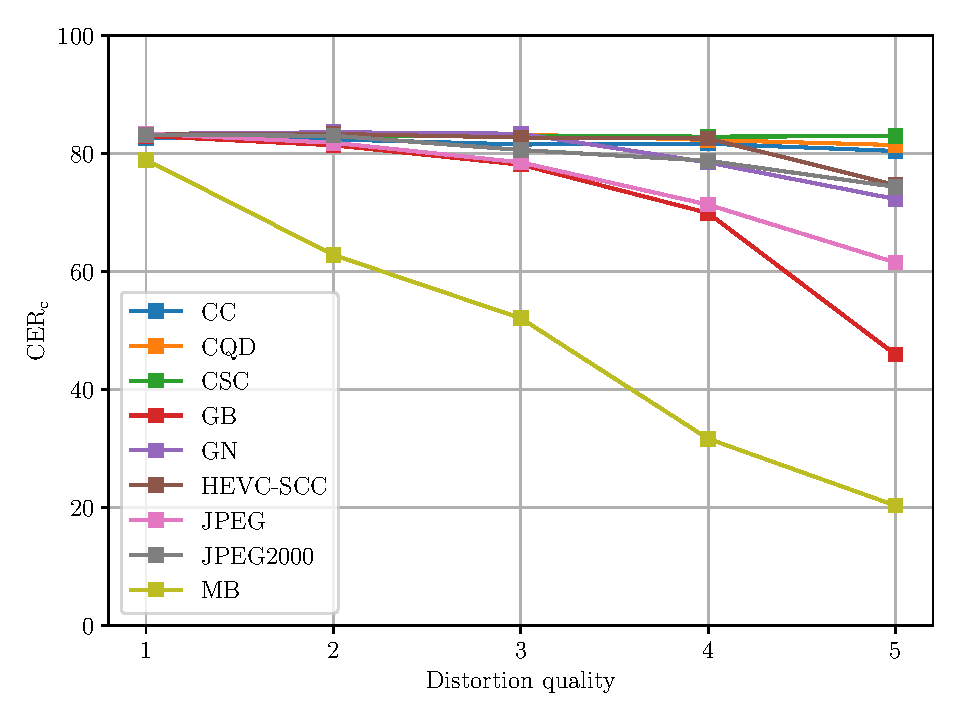
\includegraphics[width=0.9\textwidth]{../../images/analyze/cer_dist_quality_gt_ezocr.pdf}
    \caption{Mean \gls{cer} against gt for different quality levels with EasyOCR.}
\label{fig:cer_dist_quality_gt_ezocr}
\end{figure}

In \autoref{fig:cer_dist_quality_gt_ezocr} we can see the mean \gls{cer} against the gt for different quality levels with EasyOCR.

\begin{figure}[h]
\centering
    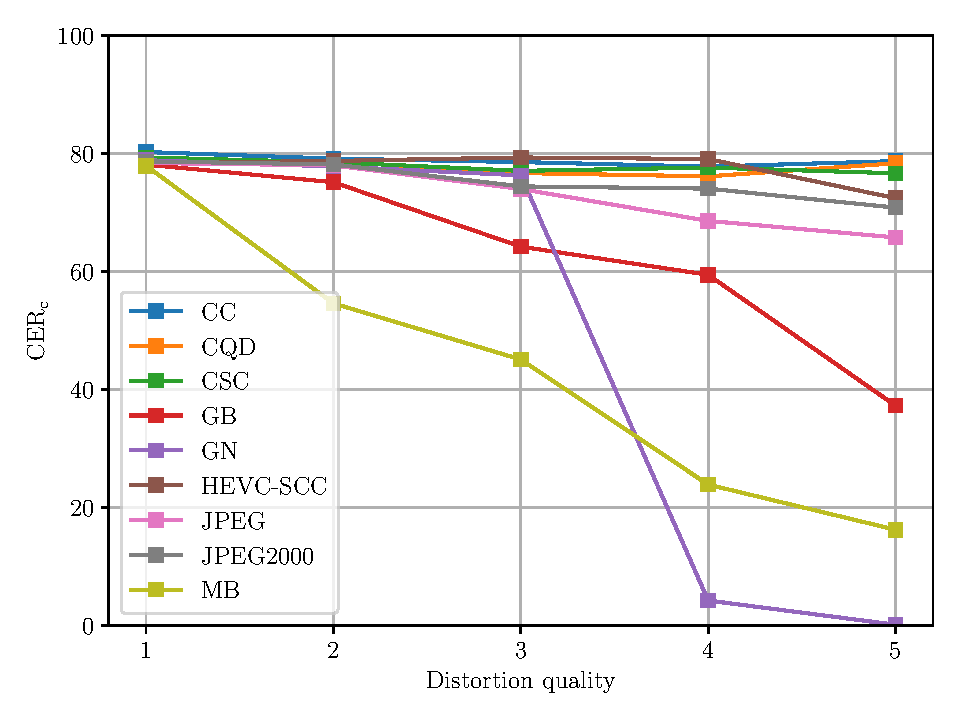
\includegraphics[width=0.9\textwidth]{../../images/analyze/cer_dist_quality_gt_tess.pdf}
    \caption{Mean \gls{cer} against gt for different quality levels with Tesseract \gls{ocr}.}
\label{fig:cer_dist_quality_gt_tesseract}
\end{figure}

In \autoref{fig:cer_dist_quality_gt_tesseract} we can see the mean \gls{cer} against the gt for different quality levels with Tesseract \gls{ocr}.

\section{Comparison against human judgement}
\label{sec:comparison_against_human_judgement}

Available datasets with subjective quality scores will be utilized to investigate
the correlation between text recognition rates and human judgement.

\begin{itemize}
\item no clear correlation, ocr not getting substantially worse with worse quality \autoref{fig:sub29} and \autoref{fig:sub3}
\item transformation via fitted model might help
\end{itemize}

\begin{figure}[h]
\centering
    \includegraphics[width=0.9\textwidth]{../../images/analyze/mos_cer_ref_sub_mean_ezocr.pdf}
    \caption{Mean \gls{cer} against mean \gls{mos} for different reference images with EasyOCR.}
\label{fig:mos_cer_ref_sub_mean_ezocr}
\end{figure}

In \autoref{fig:mos_cer_ref_sub_mean_ezocr} we can see the mean \gls{cer} against the mean \gls{mos} over selected images for all distortions with EasyOCR.

\begin{figure}[h]
\centering
    \includegraphics[width=0.9\textwidth]{../../images/analyze/mos_cer_ref_sub_mean_tess.pdf}
    \caption{Mean \gls{cer} against mean \gls{mos} for different reference images with Tesseract \gls{ocr}.}
\label{fig:mos_cer_ref_sub_mean_tesseract}
\end{figure}

In \autoref{fig:mos_cer_ref_sub_mean_tesseract} we can see the mean \gls{cer} against the mean \gls{mos} over selected images for all distortions with Tesseract \gls{ocr}.


\begin{figure}[h]
\centering
    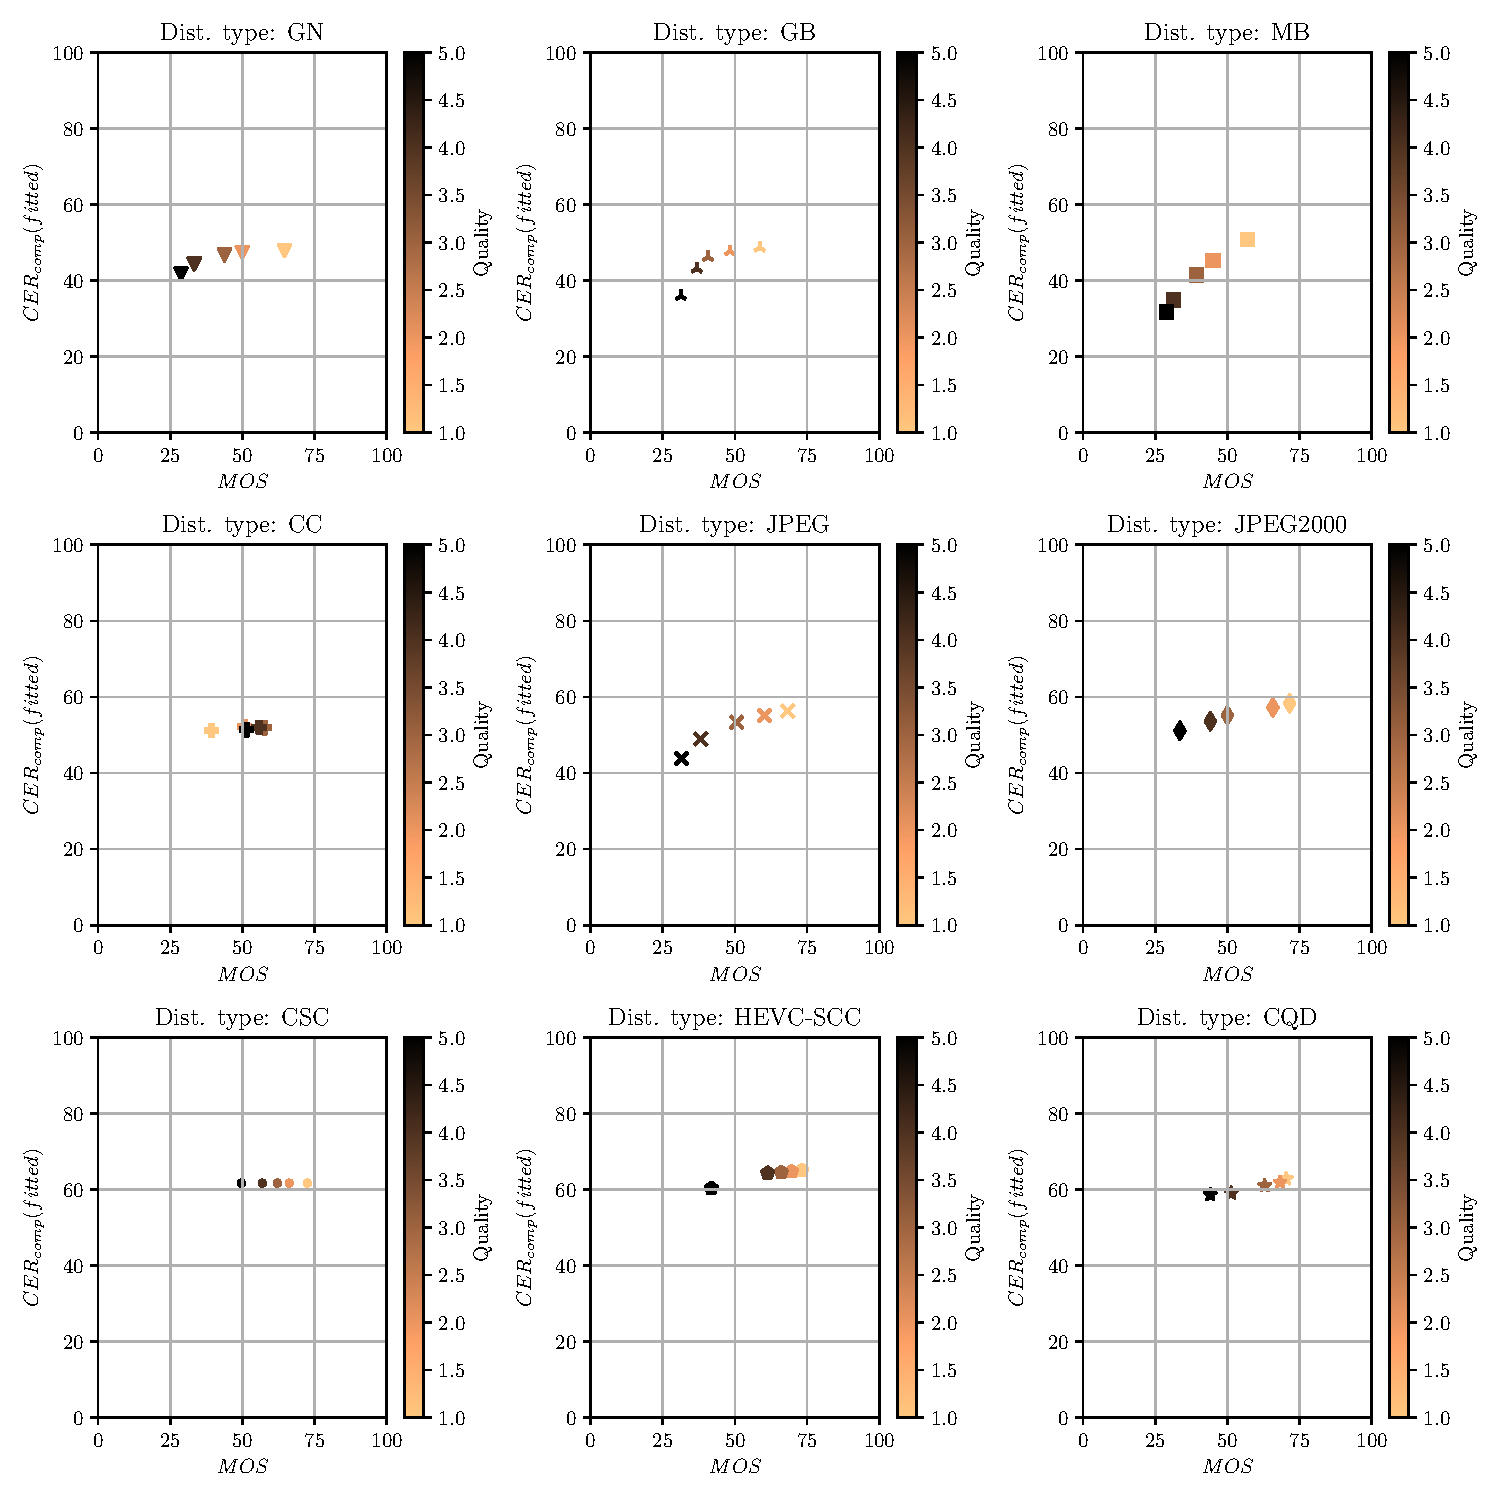
\includegraphics[width=0.9\textwidth]{../../images/analyze/mos_cer_ref_fitted_sub_mean_ezocr.pdf}
    \caption{Mean \gls{cer} (fitted) against mean \gls{mos} for different reference images with EasyOCR.}
\label{fig:mos_cer_ref_fitted_sub_mean_ezocr}
\end{figure}

In \autoref{fig:mos_cer_ref_fitted_sub_mean_ezocr} we can see the mean \gls{cer} (fitted) against the mean \gls{mos} over selected images for all distortions with EasyOCR.

\begin{figure}[h]
\centering
    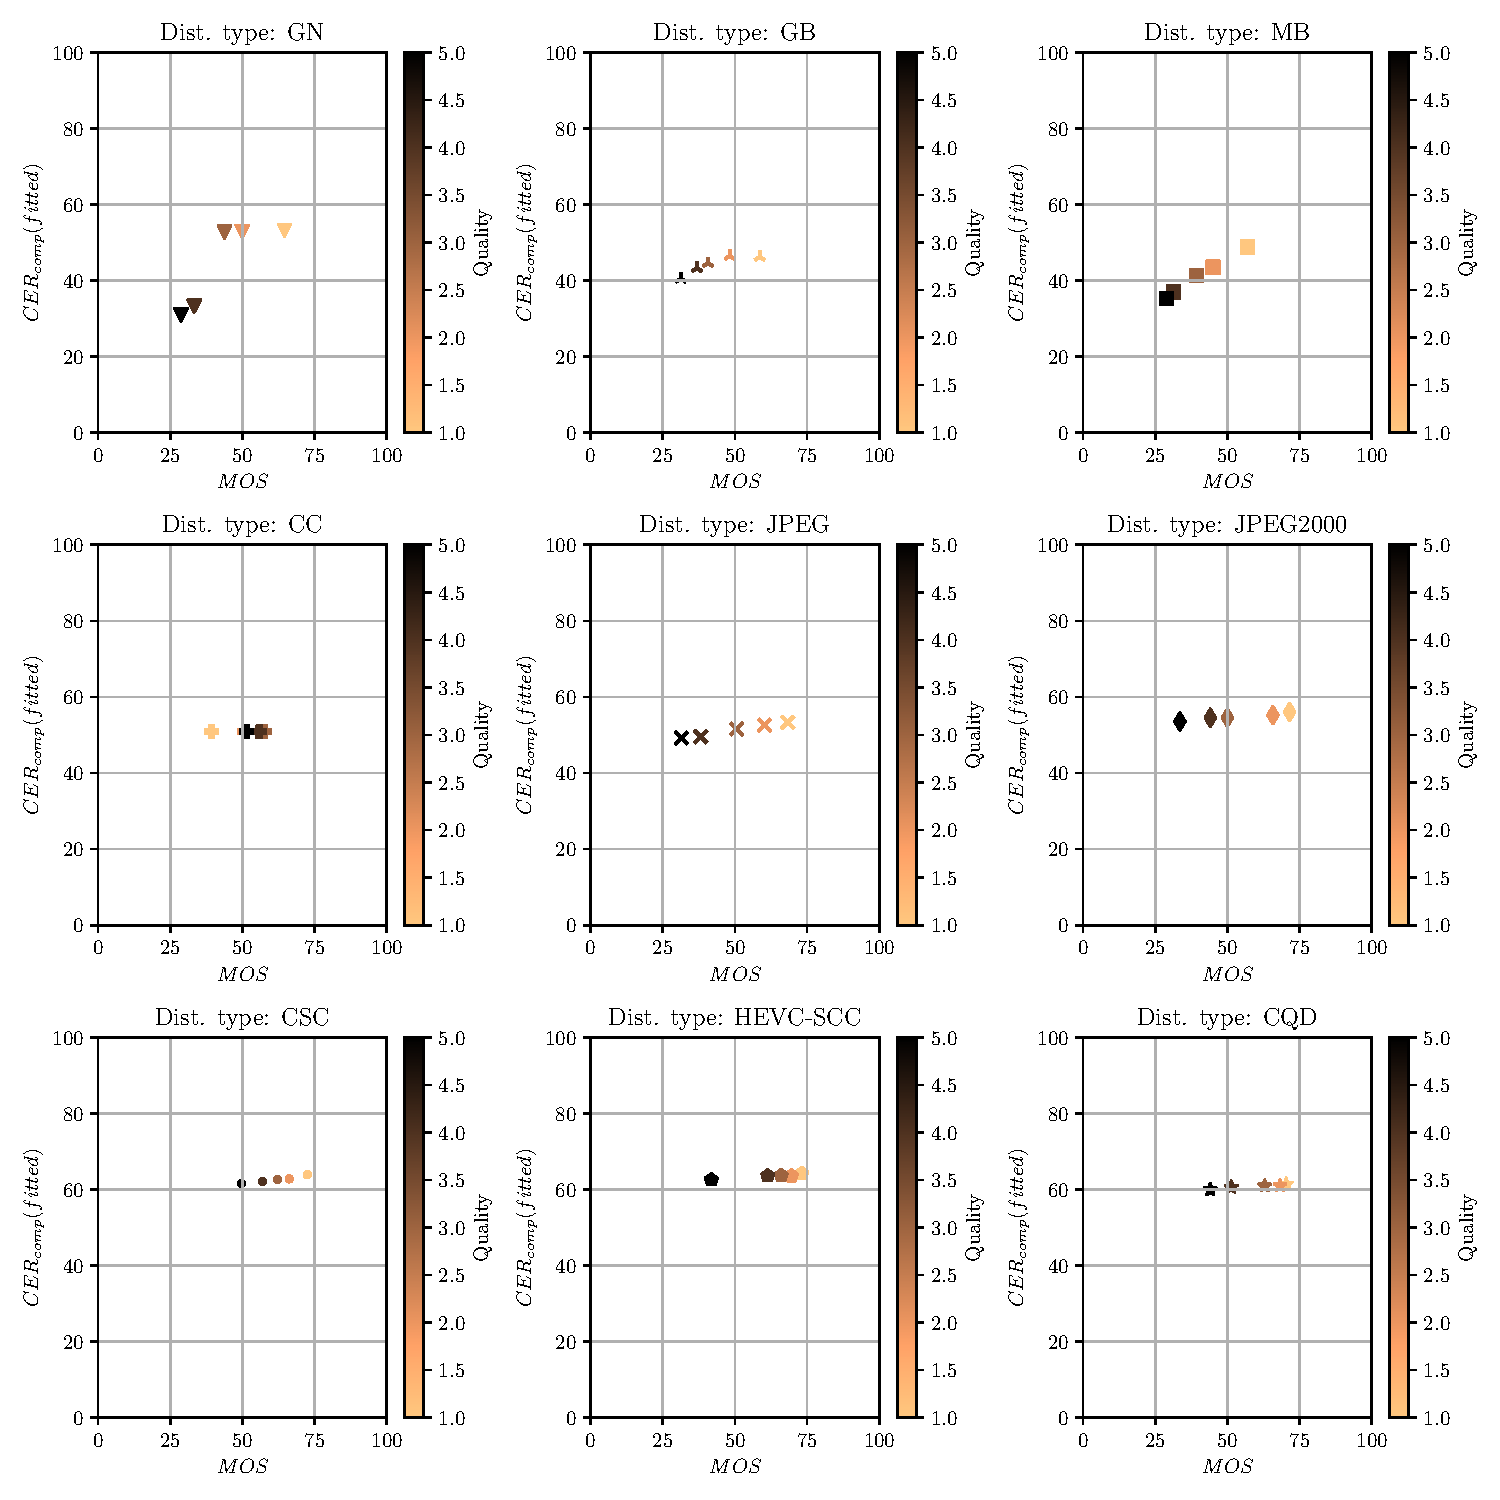
\includegraphics[width=0.9\textwidth]{../../images/analyze/mos_cer_ref_fitted_sub_mean_tess.pdf}
    \caption{Mean \gls{cer} (fitted) against mean \gls{mos} for different reference images with Tesseract \gls{ocr}.}
\label{fig:mos_cer_ref_fitted_sub_mean_tesseract}
\end{figure}

In \autoref{fig:mos_cer_ref_fitted_sub_mean_tesseract} we can see the mean \gls{cer} (fitted) against the mean \gls{mos} over selected images for all distortions with Tesseract \gls{ocr}.
    
\section{Usage of recognized text as ground truth}
\label{sec:usage_of_recognized_text_as_ground_truth}

Since most datasets do not contain textual ground truth information,
in a further step, Mr Hirt will investigate the feasibility of
using recognized text from pristine images as ground truth instead.

\begin{table}[h]
\centering
\begin{tabular}{|l|l|l|}
    \hline
    \rule{0em}{1em} \textbf{OCR Algorithm} & $\mathbf{\overline{CER}}$ & $\mathbf{\overline{CER}_{comp}}$ \\
    \hline
    EasyOCR & 0.16206 & 83.794 \\
    \hline
    Tesseract & 0.249047 & 75.0953 \\
    \hline
\end{tabular}
\caption{Mean $CER$ and $CER_{comp}$ for EasyOCR and Tesseract \gls{ocr} over selected images for reference images against \gls{gt}.}
\label{tab:mean_cer_cer_comp}
\end{table}

From \autoref{tab:mean_cer_cer_comp} we can see that EasyOCR performs better than Tesseract \gls{ocr} on the selected images.
With a $CER_{comp}$ of 83.794 its difficult to recommend using EasyOCR as a ground truth source.

\section{Codec comparison}
\label{sec:codec_comparison}
